% move all configuration stuff into includes file so we can focus on the content
\documentclass[aspectratio=169,hyperref={pdfpagelabels=false,colorlinks=true,linkcolor=white,urlcolor=blue},t]{beamer}

%%%%%%%%%%%%%%%%%%%%%%%%%%%%%%%%%%%%%%%%%%%%%%%%%%%%%%%%%%%%%%%%%%%%%%%%%%%%%%%%%%
%%%%%%%%%%%%%%%%%%%%%%%%%%%%%%%%%%%%%%%%%%%%%%%%%%%%%%%%%%%%%%%%%%%%%%%%%%%%%%%%%%
% packages
\usepackage{pict2e}
\usepackage{epic}
\usepackage{amsmath,amsfonts,amssymb}
\usepackage{units}
\usepackage{fancybox}
\usepackage[absolute,overlay]{textpos} 
\usepackage{media9} % avi2flv: "C:\Program Files\ffmpeg\bin\ffmpeg.exe" -i TuneFreqFilterbank.avi -b 600k -s 441x324 -r 15 -acodec copy TuneFreqFilterbank.flv
\usepackage{animate}
\usepackage{gensymb}
\usepackage{multirow}
\usepackage{silence}
\usepackage[backend=bibtex,style=ieee]{biblatex}
\AtEveryCitekey{\iffootnote{\tiny}{}}
\addbibresource{references}

%%%%%%%%%%%%%%%%%%%%%%%%%%%%%%%%%%%%%%%%%%%%%%%%%%%%%%%%%%%%%%%%%%%%%%%%%%%%%%%%%%
%%%%%%%%%%%%%%%%%%%%%%%%%%%%%%%%%%%%%%%%%%%%%%%%%%%%%%%%%%%%%%%%%%%%%%%%%%%%%%%%%%
% relative paths
\graphicspath{{graph/}}


%%%%%%%%%%%%%%%%%%%%%%%%%%%%%%%%%%%%%%%%%%%%%%%%%%%%%%%%%%%%%%%%%%%%%%%%%%%%%%%%%%
%%%%%%%%%%%%%%%%%%%%%%%%%%%%%%%%%%%%%%%%%%%%%%%%%%%%%%%%%%%%%%%%%%%%%%%%%%%%%%%%%%
% units
\setlength{\unitlength}{1mm}

%%%%%%%%%%%%%%%%%%%%%%%%%%%%%%%%%%%%%%%%%%%%%%%%%%%%%%%%%%%%%%%%%%%%%%%%%%%%%%%%%%
%%%%%%%%%%%%%%%%%%%%%%%%%%%%%%%%%%%%%%%%%%%%%%%%%%%%%%%%%%%%%%%%%%%%%%%%%%%%%%%%%%
% theme & layout
\usetheme{Frankfurt}
\beamertemplatenavigationsymbolsempty
%\setbeamertemplate{frametitle}[smoothbars theme]
\setbeamertemplate{frametitle}
{
    \begin{beamercolorbox}[ht=1.8em,wd=\paperwidth]{frametitle}
        \vspace{-.1em}%
        \hspace{.2em}{\strut\insertframetitle\strut}
        
        \hspace{.2em}\small\strut\insertframesubtitle\strut
        %\hfill
        %
\includegraphics[height=.8cm,keepaspectratio]{CenterMusicTechnology-solid-2lines-white-CoAtag}
        
    \end{beamercolorbox}
    \begin{textblock*}{100mm}(11.6cm,.7cm)
        \includegraphics[height=.8cm,keepaspectratio]{logo_GTCMT_black}
    \end{textblock*}
}

% set this to ensure bulletpoints without subsections
\usepackage{remreset}
\makeatletter
\@removefromreset{subsection}{section}
\makeatother
\setcounter{subsection}{1}

%---------------------------------------------------------------------------------
% appearance
\setbeamercolor{structure}{fg=gtgold}
\setbeamercovered{transparent} %invisible
\setbeamercolor{bibliography entry author}{fg=black}
\setbeamercolor*{bibliography entry title}{fg=black}
\setbeamercolor*{bibliography entry note}{fg=black}

%\usepackage{pgfpages}
%\setbeameroption{show notes}
%\setbeameroption{show notes on second screen=right}
%---------------------------------------------------------------------------------
% fontsize
\let\Tiny=\tiny

%%%%%%%%%%%%%%%%%%%%%%%%%%%%%%%%%%%%%%%%%%%%%%%%%%%%%%%%%%%%%%%%%%%%%%%%%%%%%%%%%%
%%%%%%%%%%%%%%%%%%%%%%%%%%%%%%%%%%%%%%%%%%%%%%%%%%%%%%%%%%%%%%%%%%%%%%%%%%%%%%%%%%
% warnings
\pdfsuppresswarningpagegroup=1
\WarningFilter{biblatex}{Patching footnotes failed}
\WarningFilter{latexfont}{Font shape}
\WarningFilter{latexfont}{Some font shapes}
\WarningFilter{gensymb}{Not defining}


%%%%%%%%%%%%%%%%%%%%%%%%%%%%%%%%%%%%%%%%%%%%%%%%%%%%%%%%%%%%%%%%%%%%%%%%%%%%%%%%%%
%%%%%%%%%%%%%%%%%%%%%%%%%%%%%%%%%%%%%%%%%%%%%%%%%%%%%%%%%%%%%%%%%%%%%%%%%%%%%%%%%%
% title information
\title[]{Introduction to Audio Content Analysis}   
\author[alexander lerch]{alexander lerch} 
%\institute{~}
%\date[Alexander Lerch]{}
\titlegraphic{\vspace{-16mm}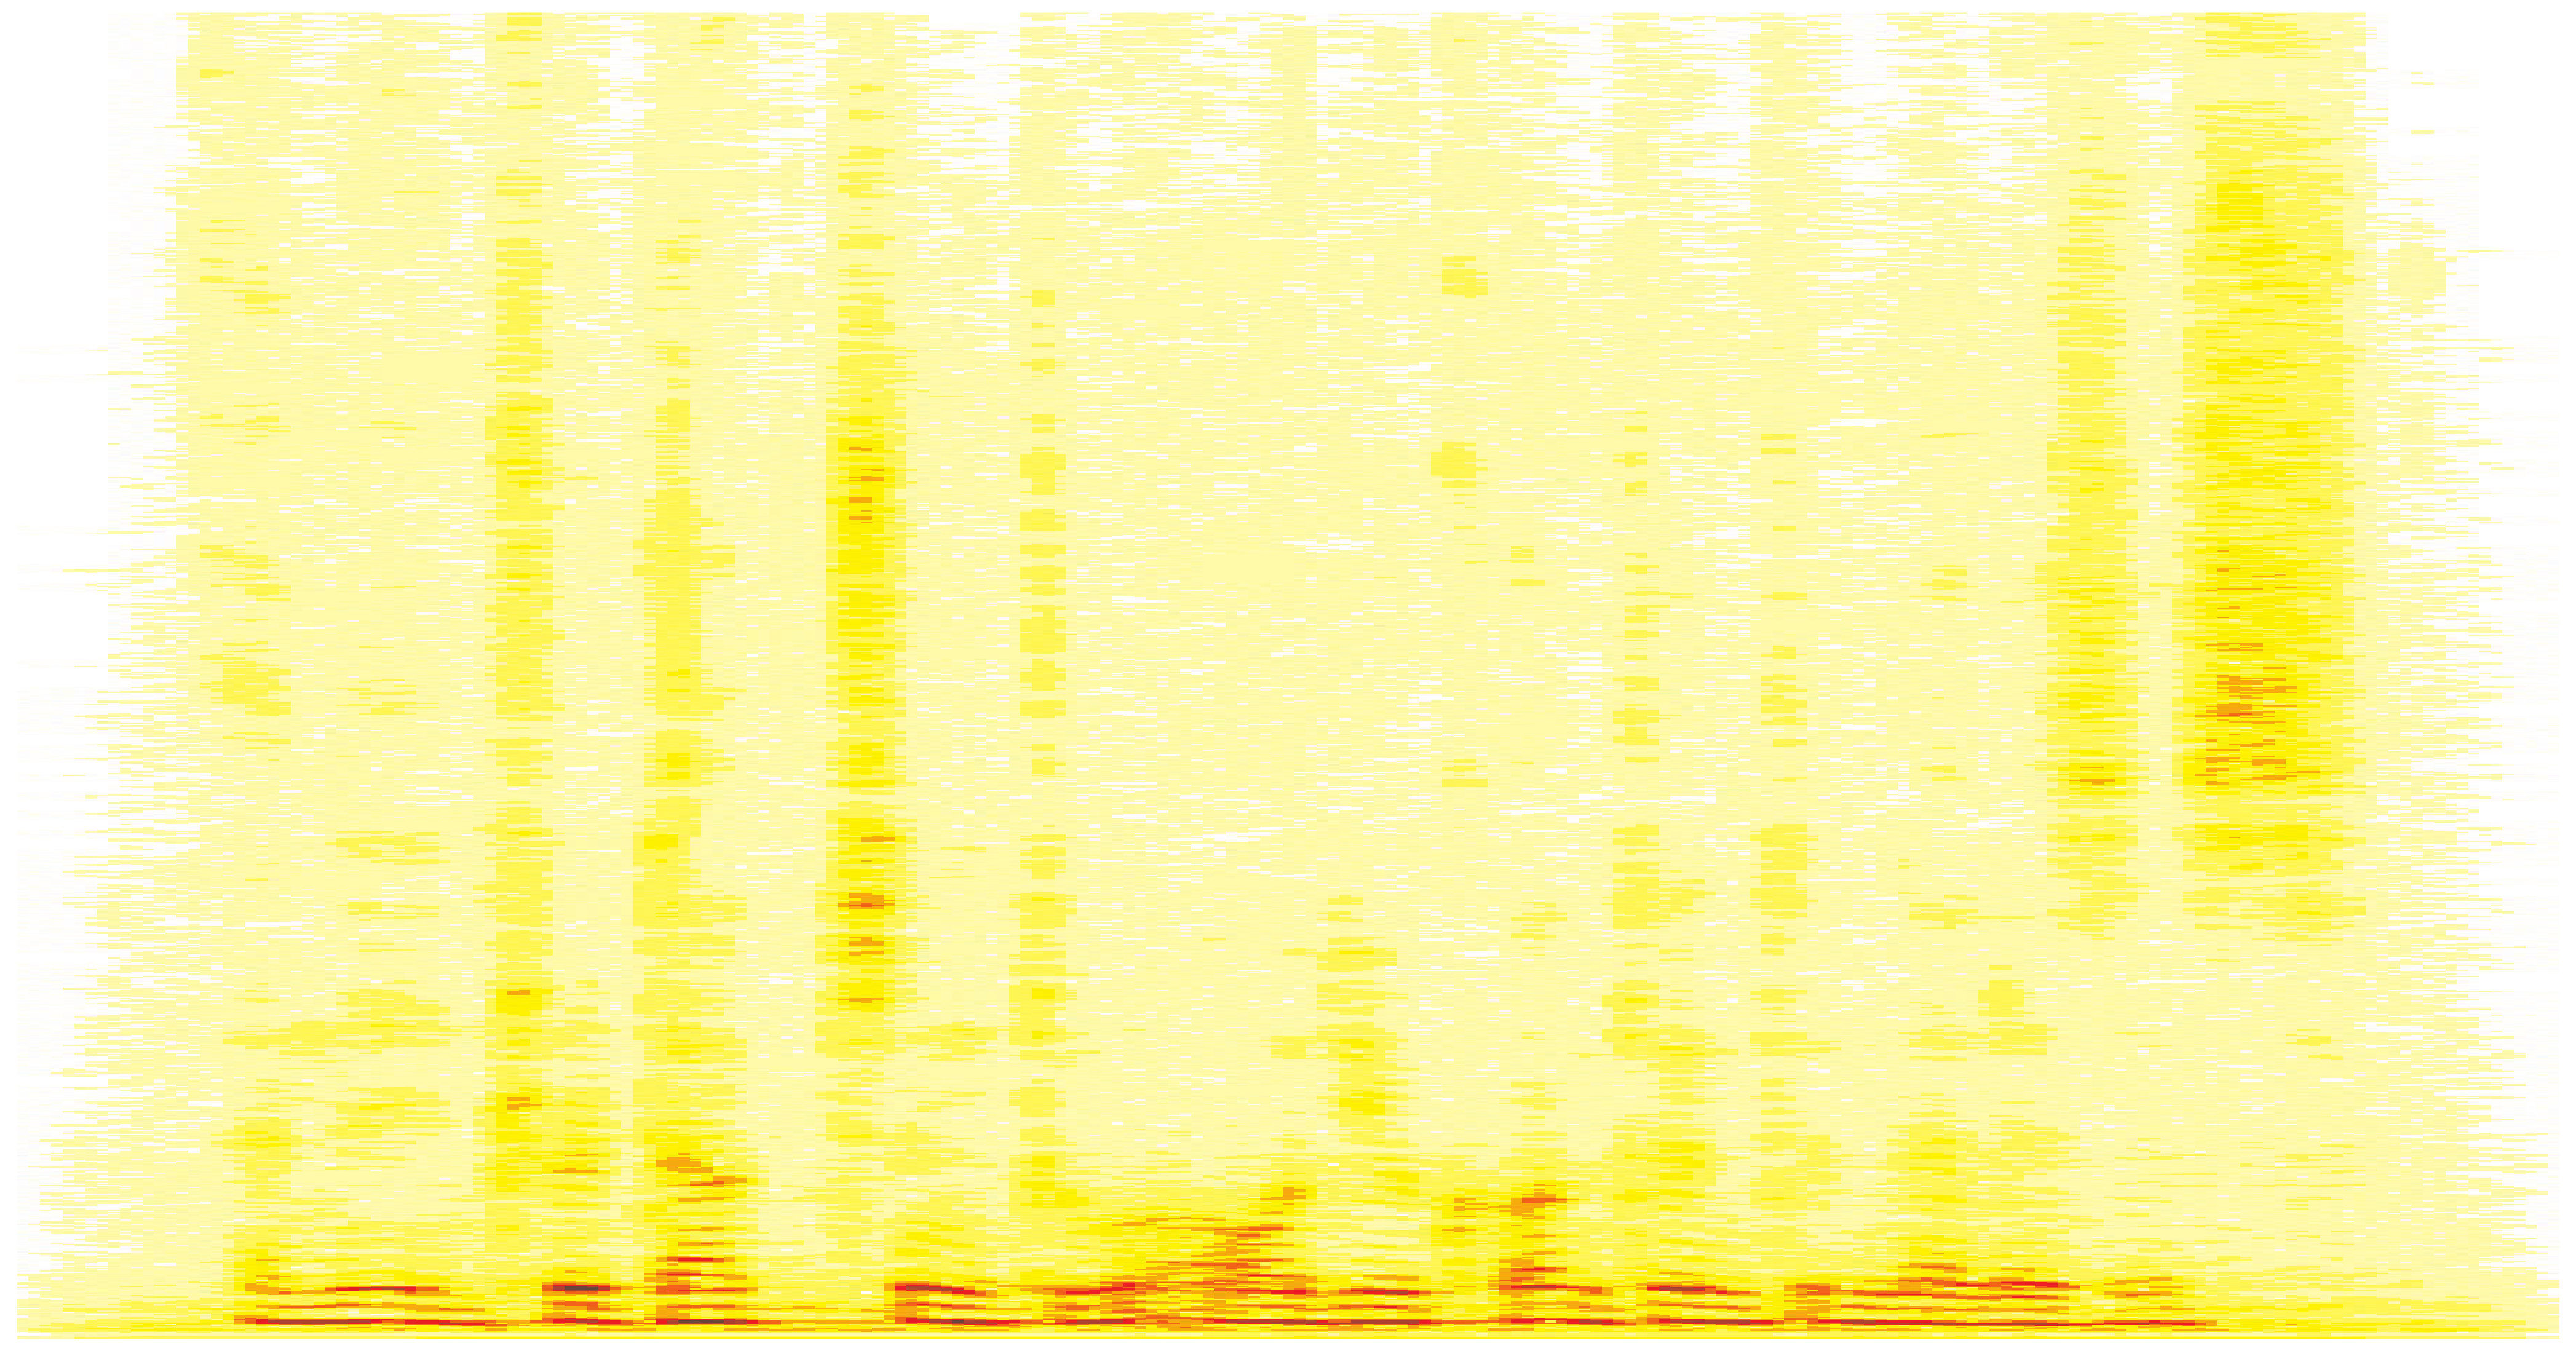
\includegraphics[width=\textwidth,height=3cm]{title}}

%%%%%%%%%%%%%%%%%%%%%%%%%%%%%%%%%%%%%%%%%%%%%%%%%%%%%%%%%%%%%%%%%%%%%%%%%%%%%%%%%%
%%%%%%%%%%%%%%%%%%%%%%%%%%%%%%%%%%%%%%%%%%%%%%%%%%%%%%%%%%%%%%%%%%%%%%%%%%%%%%%%%%
% colors
\definecolor{gtgold}{HTML}{E0AA0F} %{rgb}{0.88,0.66,1,0.06} [234, 170, 0]/256

%%%%%%%%%%%%%%%%%%%%%%%%%%%%%%%%%%%%%%%%%%%%%%%%%%%%%%%%%%%%%%%%%%%%%%%%%%%%%%%%%%
%%%%%%%%%%%%%%%%%%%%%%%%%%%%%%%%%%%%%%%%%%%%%%%%%%%%%%%%%%%%%%%%%%%%%%%%%%%%%%%%%%
% math
\DeclareMathOperator*{\argmax}{argmax}
\DeclareMathOperator*{\argmin}{argmin}
\DeclareMathOperator*{\atan}{atan}
\DeclareMathOperator*{\arcsinh}{arcsinh}
\DeclareMathOperator*{\sign}{sign}
\DeclareMathOperator*{\tcdf}{tcdf}
\DeclareMathOperator*{\si}{sinc}
\DeclareMathOperator*{\princarg}{princarg}
\DeclareMathOperator*{\arccosh}{arccosh}
\DeclareMathOperator*{\hwr}{HWR}
\DeclareMathOperator*{\flip}{flip}
\DeclareMathOperator*{\sinc}{sinc}
\DeclareMathOperator*{\floor}{floor}
\newcommand{\e}{{e}}
\newcommand{\jom}{\mathrm{j}\omega}
\newcommand{\jOm}{\mathrm{j}\Omega}
\newcommand   {\mat}[1]    		{\boldsymbol{\uppercase{#1}}}		%bold
\renewcommand {\vec}[1]    		{\boldsymbol{\lowercase{#1}}}		%bold

%%%%%%%%%%%%%%%%%%%%%%%%%%%%%%%%%%%%%%%%%%%%%%%%%%%%%%%%%%%%%%%%%%%%%%%%%%%%%%%%%%
%%%%%%%%%%%%%%%%%%%%%%%%%%%%%%%%%%%%%%%%%%%%%%%%%%%%%%%%%%%%%%%%%%%%%%%%%%%%%%%%%%
% media9
\newcommand{\includeaudio}[1]{{\includemedia[
                        addresource=audio/#1.mp3,
                        width=5mm,
                        height=5mm,
                        activate=onclick,
                        flashvars={
                            source=audio/#1.mp3  
                            &autoPlay=true
                        }]
                        {
\includegraphics[width=5mm, height=5mm]{SpeakerIcon}}
                        {APlayer.swf}}}
\newcommand{\audioautoplay}[1]{{\begin{center}\includemedia[
                            addresource=audio/#1.mp3,
                            width=.1\linewidth,
                            height=.01\linewidth,
                            activate=pageopen,
                            flashvars={
                                source=audio/#1.mp3  
                                &autoPlay=true
                            }]
                            {}
                            {APlayer.swf}\end{center}}}

\newcommand{\includevideo}[1]{{\begin{center}\includemedia[
                        addresource=video/#1.mp4,
                        width=0.8\linewidth,
                        height=0.4\linewidth,
                        activate=onclick,
                        flashvars={
                            source=video/#1.mp4  
                            &autoPlay=true
                        }]
                        {}
                        {VPlayer.swf}\end{center}}}
\newcommand{\videowithmatlab}[1]{{\begin{center}\includemedia[
                        addresource=video/animate#1.mp4,
                        width=0.8\linewidth,
                        height=0.4\linewidth,
                        activate=onclick,
                        flashvars={
                            source=video/animate#1.mp4  
                            &autoPlay=true
                        }]
                        {}
                        {VPlayer.swf}\end{center}\addreference{matlab source: matlab/animate#1.m}}}
                        

%%%%%%%%%%%%%%%%%%%%%%%%%%%%%%%%%%%%%%%%%%%%%%%%%%%%%%%%%%%%%%%%%%%%%%%%%%%%%%%%%%
%%%%%%%%%%%%%%%%%%%%%%%%%%%%%%%%%%%%%%%%%%%%%%%%%%%%%%%%%%%%%%%%%%%%%%%%%%%%%%%%%%
% other commands
\newcommand{\question}[1]{%\vspace{-4mm}
                          \setbeamercovered{invisible}
                          \begin{columns}[T]
                            \column{.8\textwidth}
                                \textbf{#1}
                            \column{.2\textwidth}
                                \vspace{-8mm}
                                \begin{flushright}
                                     
\includegraphics[scale=.5]{question_mark}
                                \end{flushright}
                                \vspace{6mm}
                          \end{columns}\pause\vspace{-12mm}}

\newcommand{\toremember}[1]{%\vspace{-4mm}
                          \begin{columns}[T]
                            \column{.8\textwidth}
                                \textbf{#1}
                            \column{.2\textwidth}
                                \vspace{-4mm}
                                \begin{flushright}
                                     
\includegraphics[scale=.5]{exclamation_mark}
                                \end{flushright}
                                \vspace{6mm}
                          \end{columns}\vspace{-6mm}}

\newcommand{\matlabexercise}[1]{%\vspace{-4mm}
                          \setbeamercovered{invisible}
                          \begin{columns}[T]
                            \column{.8\textwidth}
                                \textbf{matlab exercise}: #1
                            \column{.2\textwidth}
                                \begin{flushright}
                                     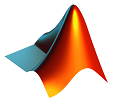
\includegraphics[scale=.5]{logo_matlab}
                                \end{flushright}
                                %\vspace{6mm}
                          \end{columns}}

\newcommand{\addreference}[1]{  
                  
                    \begin{textblock*}{\baselineskip }(1.12\textwidth,.3\textheight) %(1.15\textwidth,.4\textheight)
                        \rotatebox{90}{\tiny {#1}}
                    \end{textblock*}}
                    
\newcommand{\figwithmatlab}[1]{
                    \begin{figure}
                        \centering
                        \includegraphics{#1}
                        %\label{fig:#1}
                    \end{figure}
                    
                    \addreference{matlab source: \href{https://github.com/alexanderlerch/ACA-Slides/blob/master/matlab/display#1.m}{matlab/display#1.m}}}
\newcommand{\figwithref}[2]{
                    \begin{figure}
                        \centering
                        \includegraphics{#1}
                        \label{fig:#1}
                    \end{figure}
                    
                    \addreference{#2}}  
                                    
\newcommand{\inserticon}[1]{

                    \begin{textblock*}{100mm}(14.5cm,7.5cm)
                        \includegraphics[height=.8cm,keepaspectratio]{#1}
                    \end{textblock*}}            

%%%%%%%%%%%%%%%%%%%%%%%%%%%%%%%%%%%%%%%%%%%%%%%%%%%%%%%%%%%%%%%%%%%%%%%%%%%%%%%%%%
%%%%%%%%%%%%%%%%%%%%%%%%%%%%%%%%%%%%%%%%%%%%%%%%%%%%%%%%%%%%%%%%%%%%%%%%%%%%%%%%%%
% counters
\newcounter{i}
\newcounter{j}
\newcounter{iXOffset}
\newcounter{iYOffset}
\newcounter{iXBlockSize}
\newcounter{iYBlockSize}
\newcounter{iYBlockSizeDiv2}
\newcounter{iDistance}



\subtitle{Module 6.2: Tempo Detection}

%%%%%%%%%%%%%%%%%%%%%%%%%%%%%%%%%%%%%%%%%%%%%%%%%%%%%%%%%%%%%%%%%%%%%%%%%%%%
\begin{document}
    % generate title page
	

\begin{frame}
    \titlepage
    %\vspace{-5mm}
    \begin{flushright}
        \href{http://www.gtcmt.gatech.edu}{\includegraphics[height=.8cm,keepaspectratio]{logo_GTCMT_black}}
    \end{flushright}
\end{frame}


    \section[overview]{lecture overview}
        \begin{frame}{introduction}{overview}
            \begin{block}{corresponding textbook section}
                    \href{http://ieeexplore.ieee.org/xpl/articleDetails.jsp?arnumber=6331122}{Chapter 6~---~Temporal Analysis}: pp.~146--148
            \end{block}

            \begin{itemize}
                \item   \textbf{lecture content}
                    \begin{itemize}
                        \item   introduction to tempo detection and beat tracking
                        \item   overview over basic approaches
                        \item    typical challenges
                    \end{itemize}
                \bigskip
                \item<2->   \textbf{learning objectives}
                    \begin{itemize}
                        \item   discuss advantages and disadvantages for different approaches to tempo detection and beat tracking
                        \item   summarize the typical challenges of beat tracking systems
                    \end{itemize}
            \end{itemize}
            \inserticon{directions}
        \end{frame}

    \section[intro]{introduction}
        \begin{frame}{tempo detection \& beat tracking}{problem statement}
            \begin{itemize}
                \item   \textbf{tempo detection}
                    \begin{itemize}
                        \item   detect speed of regular pulse (foot-tapping rate)
                    \end{itemize}
                \bigskip
                \item   \textbf{beat tracking}
                    \begin{itemize}
                        \item   detect the time instances the tempo pulses occur (beat phase)
                    \end{itemize}
            \end{itemize}
        \end{frame}
        
       \begin{frame}{tempo detection \& beat tracking}{introduction}
            \begin{itemize}
                \item \textbf{objectives}
                    \begin{enumerate}
                        \item	find the tempo from the novelty function/onsets
                        \item	find the beat locations
                    \end{enumerate}
                \bigskip
                \item \textbf{systematic problems}:
                    \begin{enumerate}
                        \item	distinguish \textit{hierarchical levels}
                            \begin{itemize}
                                \item[]	
                                \item	meter
                                \item	beat
                                \item	subbeat/tatum
                            \end{itemize}
                            \vspace{-17mm}
                            \begin{flushright}
                                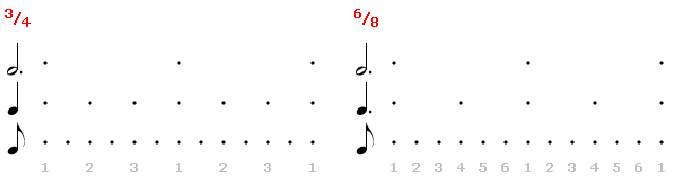
\includegraphics[scale=.25]{graph/periodiclevels}
                            \end{flushright}
                        \item<1->	detect \textit{beats without onsets}
                        \item<1->	recognize \textit{onsets without beats}
                    \end{enumerate}
            \end{itemize}
        \end{frame}

    \section{oscillator approach}
        \begin{frame}{tempo detection \& beat tracking}{oscillator approach}
            \textbf{Beat tracking with an oscillator}\footfullcite{large_beat_1995}
            \begin{figure}
                \centering
                    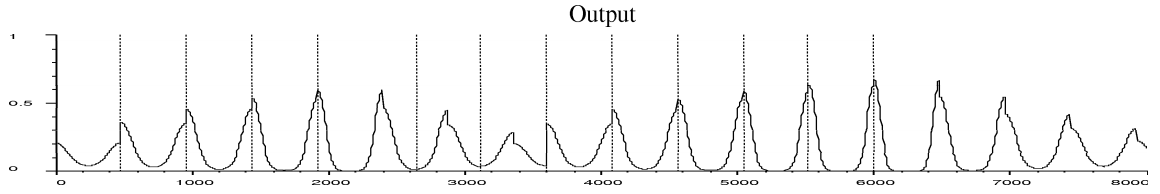
\includegraphics[scale=.3]{graph/BPM_large_oscillator}
            \end{figure}
            
            \begin{enumerate}
                \item	initialize pulse generator (tempo estimate, beat position estimate)
                \item<2->	predict next beat location with pulse
                \item<3->	adapt acc.\ to distance (predicted vs.\ real onset position)
                    \begin{itemize}
                        \item	beat period
                        \item	beat phase
                    \end{itemize}
                \item<4->	predict with adapted settings
                \item<4->   adapt \ldots
            \end{enumerate}
        \end{frame}
        \begin{frame}{tempo detection \& beat tracking}{oscillator approach: initialization}
            \question{How to estimate the initial tempo}

            \begin{itemize}
                \item	location of maximum of \textbf{ACF of novelty function}
                \item<2->	maximum of \textbf{IOI histogram}
                    \begin{figure}
                        \centering
                            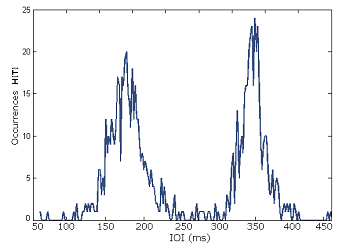
\includegraphics[scale=.3]{graph/ioi_hist}
                    \end{figure}
                \item<2->	maximum of \textbf{beat spectrum/histogram}
                \item<2->	\ldots
            \end{itemize}
        \end{frame}
        \begin{frame}{tempo detection \& beat tracking}{multi-agent approach}
            \begin{enumerate}
                \item	run \textbf{multiple beat trackers} with different parameters
                    \begin{itemize}
                        \item	initial tempo
                        \item	initial beat phase
                        \item	adaptation speed
                    \end{itemize}
                \item<2->	compute reliability/confidence criteria:
                
                    \begin{itemize}
                        \item	match beat and onset times
                        \item<3->	tempo stability
                        \item<4->	majority of different agents
                        \item   \ldots
                    \end{itemize}
                \item<5->	choose\textbf{ most reliable agent} (or path between agents)
            \end{enumerate}
        \end{frame}
        
    \section{filterbank approach}
        \begin{frame}{tempo detection \& beat tracking}{filterbank approach}
            \begin{columns}[T]
            \column{.5\linewidth}
                \begin{enumerate}
                    \item	design \textbf{filterbank} (e.g. comb resonators spaced 1 beat)
                    \item<2->	compute filter output energy	
                    \item<3->	pick maximum
                \end{enumerate}
            \column{.5\linewidth}
                \only<1>{
                \begin{figure}
                    \centering
                        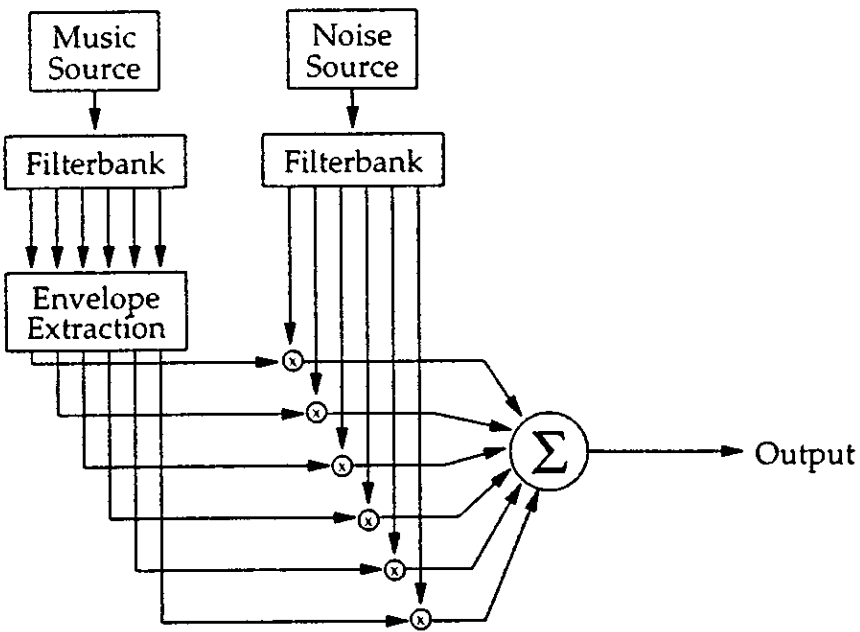
\includegraphics[scale=.25]{graph/BPM_Scheirer_filterbank}
                \end{figure}
                }
                \only<2->{
                \begin{figure}
                    \centering
                        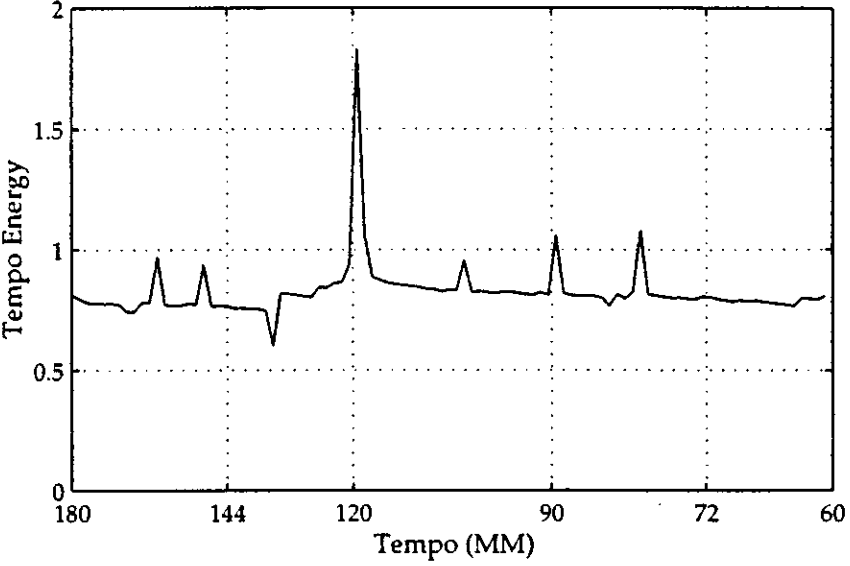
\includegraphics[scale=.25]{graph/BPM_Scheirer_beatspectrum}
                \end{figure}
                }
            \end{columns}
            plots by Scheirer\footfullcite{scheirer_tempo_1998}
        \end{frame}

    \section{template approach}
        \begin{frame}{tempo detection \& beat tracking}{template-based approach}
            \begin{enumerate}
                \item	define set of \textbf{template pulses} in all tempi
                \smallskip
                \item<1->	compute CCF between novelty function (or its ACF) and all templates
                \smallskip
                \item<1->	choose template with highest correlation as tempo
                \smallskip
                \item<1->	choose lag with highest correlation as beat phase
            \end{enumerate}
        \end{frame}

    \section{challenges}
        \begin{frame}{tempo detection \& beat tracking}{typical problems}
            \begin{enumerate}
                \item	tempo: detection of \textbf{double/half tempo} (triple, \ldots)
                \smallskip
                \item<1->	phase: detection of \textbf{off-beats}
                \smallskip
                \item<1->	tempo \& phase: strongly depends on \textbf{initialization values}
                \smallskip
                \item<1->	tempo \& phase: only \textbf{slow adaptation} --- no sudden tempo changes
            \end{enumerate}
            
            challenges with adaptation speed example:                     \includeaudio{sonata-ck330_auftakt}
        \end{frame}
        %\begin{frame}{tempo detection \& beat tracking}{evaluation}
            %\question{how do you properly evaluate a tempo detection or beat tracking system}
            %\begin{itemize}
                %\item   methodology
                %\smallskip
                %\item   ground truth
                    %\begin{itemize}
                        %\item   how to get/generate
                        %\item   necessary annotations
                    %\end{itemize}
                %\smallskip
                %\item   metrics
                    %\begin{itemize}
                        %\item   how to measure the accuracy of your system
                    %\end{itemize}
            %\end{itemize}
        %\end{frame}
    
    \section{summary}
        \begin{frame}{summary}{lecture content}
            \begin{itemize}
                \item   \textbf{tempo analysis}
                    \begin{itemize}
                        \item   similar to pitch detection on a different scale
                            \begin{itemize}
                                \item   periodicity analysis of novelty function
                                \item   time or spectral domain
                            \end{itemize}
                    \end{itemize}
                \bigskip
                \item   \textbf{typical approaches}
                    \begin{itemize}
                        \item   oscillator
                        \item   histogram/beat spectrum
                        \item   template correlation
                    \end{itemize}
                \bigskip
                \item   \textbf{main challenges}
                    \begin{itemize}
                        \item   double/half tempo
                        \item   adaptation to sudden tempo changes
                    \end{itemize}
            \end{itemize}
            \inserticon{summary}
        \end{frame}
\end{document}
